\section*{Contador}

\exercise~Qual entrada dos flip-flops é utilizada para reiniciar a contagem em
um circuito contador?

\exercise~Projete um contador síncrono de três bits para fazer a
contagem crescente ou decrescente através de uma variável de controle.

\exercise~No circuito da Figura~\ref{fig:counter}, o clock é um sinal
alternado entre os níveis lógicos alto e baixo, com frequência de
1kHz. Qual o tempo necessário para este contador, iniciando todas as
saídas Q em $0$, reiniciar a contagem novamente?

\begin{figure}[ht]
  \centering  
  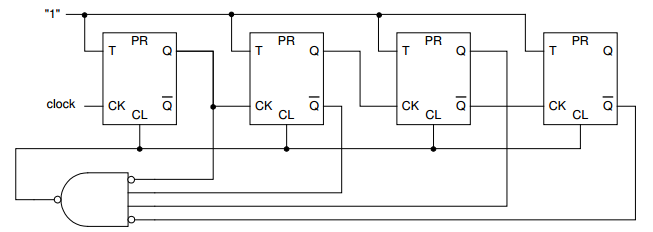
\includegraphics[scale=.5]{\imgdir/async-counter-4bit.png}
  \caption{Contador assíncrono.}
  \label{fig:counter}
\end{figure}

\exercise~Tempo de propagação é o tempo que um flip-flop demora para
alterar a saída Q quando recebe um clock de atualização. Considere um
Flip-Flop JK com tempo de propagação igual a 300ns.  

Em um contador assíncrono que conta de 0 a 15 qual o tempo mínimo que
deve ser esperado para ler a saída após um pulso de clock? E em um
contador síncrono?
